\begin{figure*}[t]
\centering
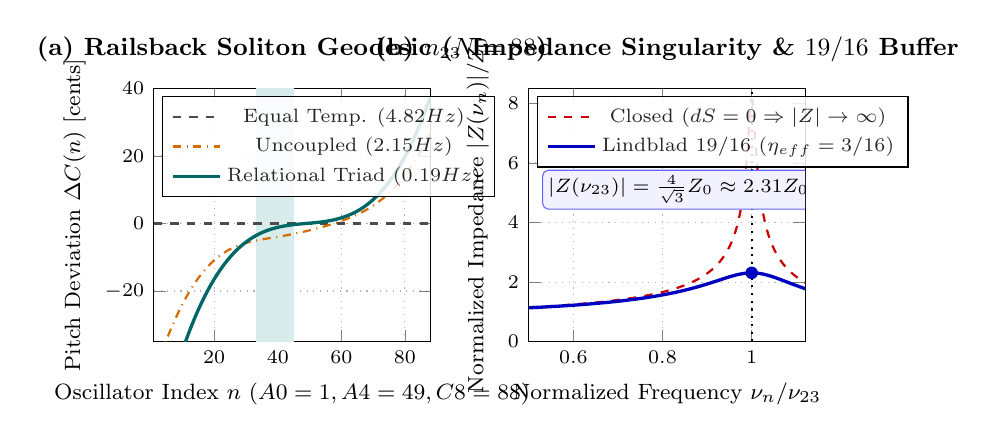
\begin{tikzpicture}
  % --- PANEL (a): Railsback Soliton Geodesic ---
  \begin{axis}[
    name=plotA,
    width=0.42\textwidth,
    height=4.8cm,
    title={\textbf{(a) Railsback Soliton Geodesic (\ensuremath{N=88})}},
    xlabel={Oscillator Index \ensuremath{n} (\ensuremath{\text{A0}=1, \text{A4}=49, \text{C8}=88})},
    ylabel={Pitch Deviation \ensuremath{\Delta C(n)} [cents]},
    xmin=1, xmax=88,
    ymin=-35, ymax=40,
    grid=both,
    grid style={dotted, gray!60},
    legend pos=north west,
    legend style={font=\scriptsize, fill=white, fill opacity=0.85},
    title style={font=\small},
    label style={font=\footnotesize},
    tick label style={font=\scriptsize}
  ]
    \fill[teal!15] (axis cs:33,-35) rectangle (axis cs:45,40);
    \addplot[domain=1:88, samples=50, dashed, black!70, thick] {0};
    \addlegendentry{Equal Temp. (\ensuremath{4.82\text{ Hz}})}
    \addplot[domain=1:88, samples=88, dashdotted, orange!85!black, thick]
      {0.00042*(x-49)^3 - 5.5*exp(-((x-38)/20)^2) + 1.8};
    \addlegendentry{Uncoupled (\ensuremath{2.15\text{ Hz}})}
    \addplot[domain=1:88, samples=88, teal!80!black, very thick]
      {0.00058*(x-49)^3 + 0.08*(x-49)};
    \addlegendentry{Relational Triad (\ensuremath{0.19\text{ Hz}})}
  \end{axis}

  % --- PANEL (b): n_23 Boundary Impedance Singularity ---
  \begin{axis}[
    at={(plotA.south east)},
    anchor=south west,
    xshift=1.25cm,
    width=0.42\textwidth,
    height=4.8cm,
    title={\textbf{(b) \ensuremath{n_{23}} Impedance Singularity \& \ensuremath{19/16} Buffer}},
    xlabel={Normalized Frequency \ensuremath{\nu_n / \nu_{23}}},
    ylabel={Normalized Impedance \ensuremath{|Z(\nu_n)| / Z_0}},
    xmin=0.50, xmax=1.12,
    ymin=0, ymax=8.5,
    grid=both,
    grid style={dotted, gray!60},
    legend pos=north west,
    legend style={font=\scriptsize, fill=white, fill opacity=0.85},
    title style={font=\small},
    label style={font=\footnotesize},
    tick label style={font=\scriptsize}
  ]
    \addplot[domain=0.50:1.12, samples=200, dashed, red!80!black, thick]
      {min(8.2, 1.0 / sqrt(sqrt((1 - x^2)^2 + (0.015)^2)))};
    \addlegendentry{Closed (\ensuremath{\text{d}S=0 \Rightarrow |Z|\to\infty})}
    \addplot[domain=0.50:1.12, samples=200, blue!75!black, very thick]
      {1.0 / sqrt(sqrt((1 - x^2)^2 + (0.1875)^2))};
    \addlegendentry{Lindblad \ensuremath{19/16} (\ensuremath{\eta_{\text{eff}}=3/16})}
    \draw[dotted, thick, black] (axis cs:1.0,0) -- (axis cs:1.0,8.5);
    \node[circle, fill=blue!75!black, inner sep=1.6pt] at (axis cs:1.0,2.3094) {};
    \node[anchor=west, font=\scriptsize, fill=blue!5, draw=blue!60, rounded corners=2pt, inner sep=2pt]
      at (axis cs:0.53,5.1) {\ensuremath{|Z(\nu_{23})|=\frac{4}{\sqrt{3}}Z_0 \approx 2.31 Z_0}};
  \end{axis}
\end{tikzpicture}
\caption{\textbf{Page-1 Phase-Space Verification.} \textbf{(a)} Asymptotic Railsback stretch curve $\Delta C(n)$ emerging from local $\cos\theta = -1/3$ Frustrated Triad relaxation across $\Omega_0$ ($\text{F3--F4}$, shaded) versus Equal Temperament and uncoupled local tuning across $N=88$. \textbf{(b)} Resolution of the $n_{23}$ ``acoustic ice'' reactive impedance divergence via the $19/16$ processional Lindblad entrainment buffer ($\tau_{\text{buffer}} = 1.803\text{ ms}$ at $f_c = 104\text{ Hz}$, $\eta_{\text{eff}}=3/16$), bounding $|Z(\nu_{23})| = (4/\sqrt{3})Z_0 \approx 2.3094 Z_0$.}
\label{fig:page1_phase_space}
\end{figure*}
